\documentclass[light]{lutbeamer} % change between light and dark for the background
%\documentclass[t]{lutbeamer} % use "t" option for top alignment 
\usepackage{comment}
\usepackage{qrcode}

\usepackage{pgfpages}
\setbeameroption{hide notes} % Only slides
% \setbeameroption{show only notes} % Only notes
% \setbeameroption{show notes on second screen=right} % Both

\setdepartment{Ceramics for the built environment}
\institute[]{}
\author{}
\title[Zitadelle Spandau]{Zitadelle Spandau}
\subtitle{Ceramics in the build environment}
\date{\today}


\begin{document}

% front page
{ % all template changes are local to this group.
    \setbeamertemplate{navigation symbols}{}
    \begin{frame}<article:0>[plain,noframenumbering]
        \begin{tikzpicture}[remember picture,overlay]
            \node[at=(current page.center)] {
                \includegraphics[
                                 width=\paperwidth,
                                 height=\paperheight]{figures/frontpage_figure}
            };
        \end{tikzpicture}
    \end{frame}
}

% Outline
\begin{comment}
    \AtBeginSection[]
{
\begin{frame}[plain,noframenumbering]
\frametitle{Outline}
\begin{columns}[T]
    \begin{column}{0.01\textwidth}
        
    \end{column}
    \begin{column}{0.95\textwidth}
        \tableofcontents[currentsection,
                        %currentsubsection,
                        %hideothersubsections, 
                        %sectionstyle=show/shaded, 
                        %subsectionstyle=show/shaded%/hide
                 ]
    \end{column}
\end{columns}
\end{frame}
}
\end{comment}



% use blurred background figure
% {\usebackgroundtemplate{%
% \begin{tikzpicture}[remember picture,overlay]
% \node [anchor=south east, 
%       xshift=2.15cm, 
%       yshift=0.25cm,
%       opacity=0.35, scale=0.3]  at (current page.south east)  {\includegraphics{figures/figurename}};
% \end{tikzpicture}
% }
\begin{comment}
{ % title page
\begin{frame}[plain]
\maketitle
\small
\par\vskip0.5em
{\footnotesize
    \hspace*{0.2cm}
    \begin{tabular}[t]{@{}l@{\hspace{3pt}}p{.5\textwidth}@{}}
    Supervisor: & Prof. Supervisor, University
    \end{tabular}%
    \par\vskip0.5em
    \hspace*{0.26cm}\begin{tabular}[t]{@{}l@{\hspace{3pt}}p{.5\textwidth}@{}}
    Opponent: & Prof. Opponent, University
    \end{tabular}%
    }
\note[item]{
Honored custos, honored opponent, honored listeners, ...
}
\end{frame}
}
\end{comment}


\section{Motivation}
\subsection{Spandau - Old city}
\begin{frame}
\frametitle{Motivation}
\framesubtitle{}
\vspace{5mm}
\begin{figure}
    \centering
        \includegraphics[height=0.65\paperheight]{figures/maps/map_spandau_detail.png}
        \caption{Altstadt Spandau and Zitadelle \cite{OpenStreetMap}}
    \label{fig:enter-label}
\end{figure}

\end{frame}

\begin{frame}{Impressionen Spandau}
\vspace{0.5cm}
    \begin{columns}
        \begin{column}{0.3\textwidth}
            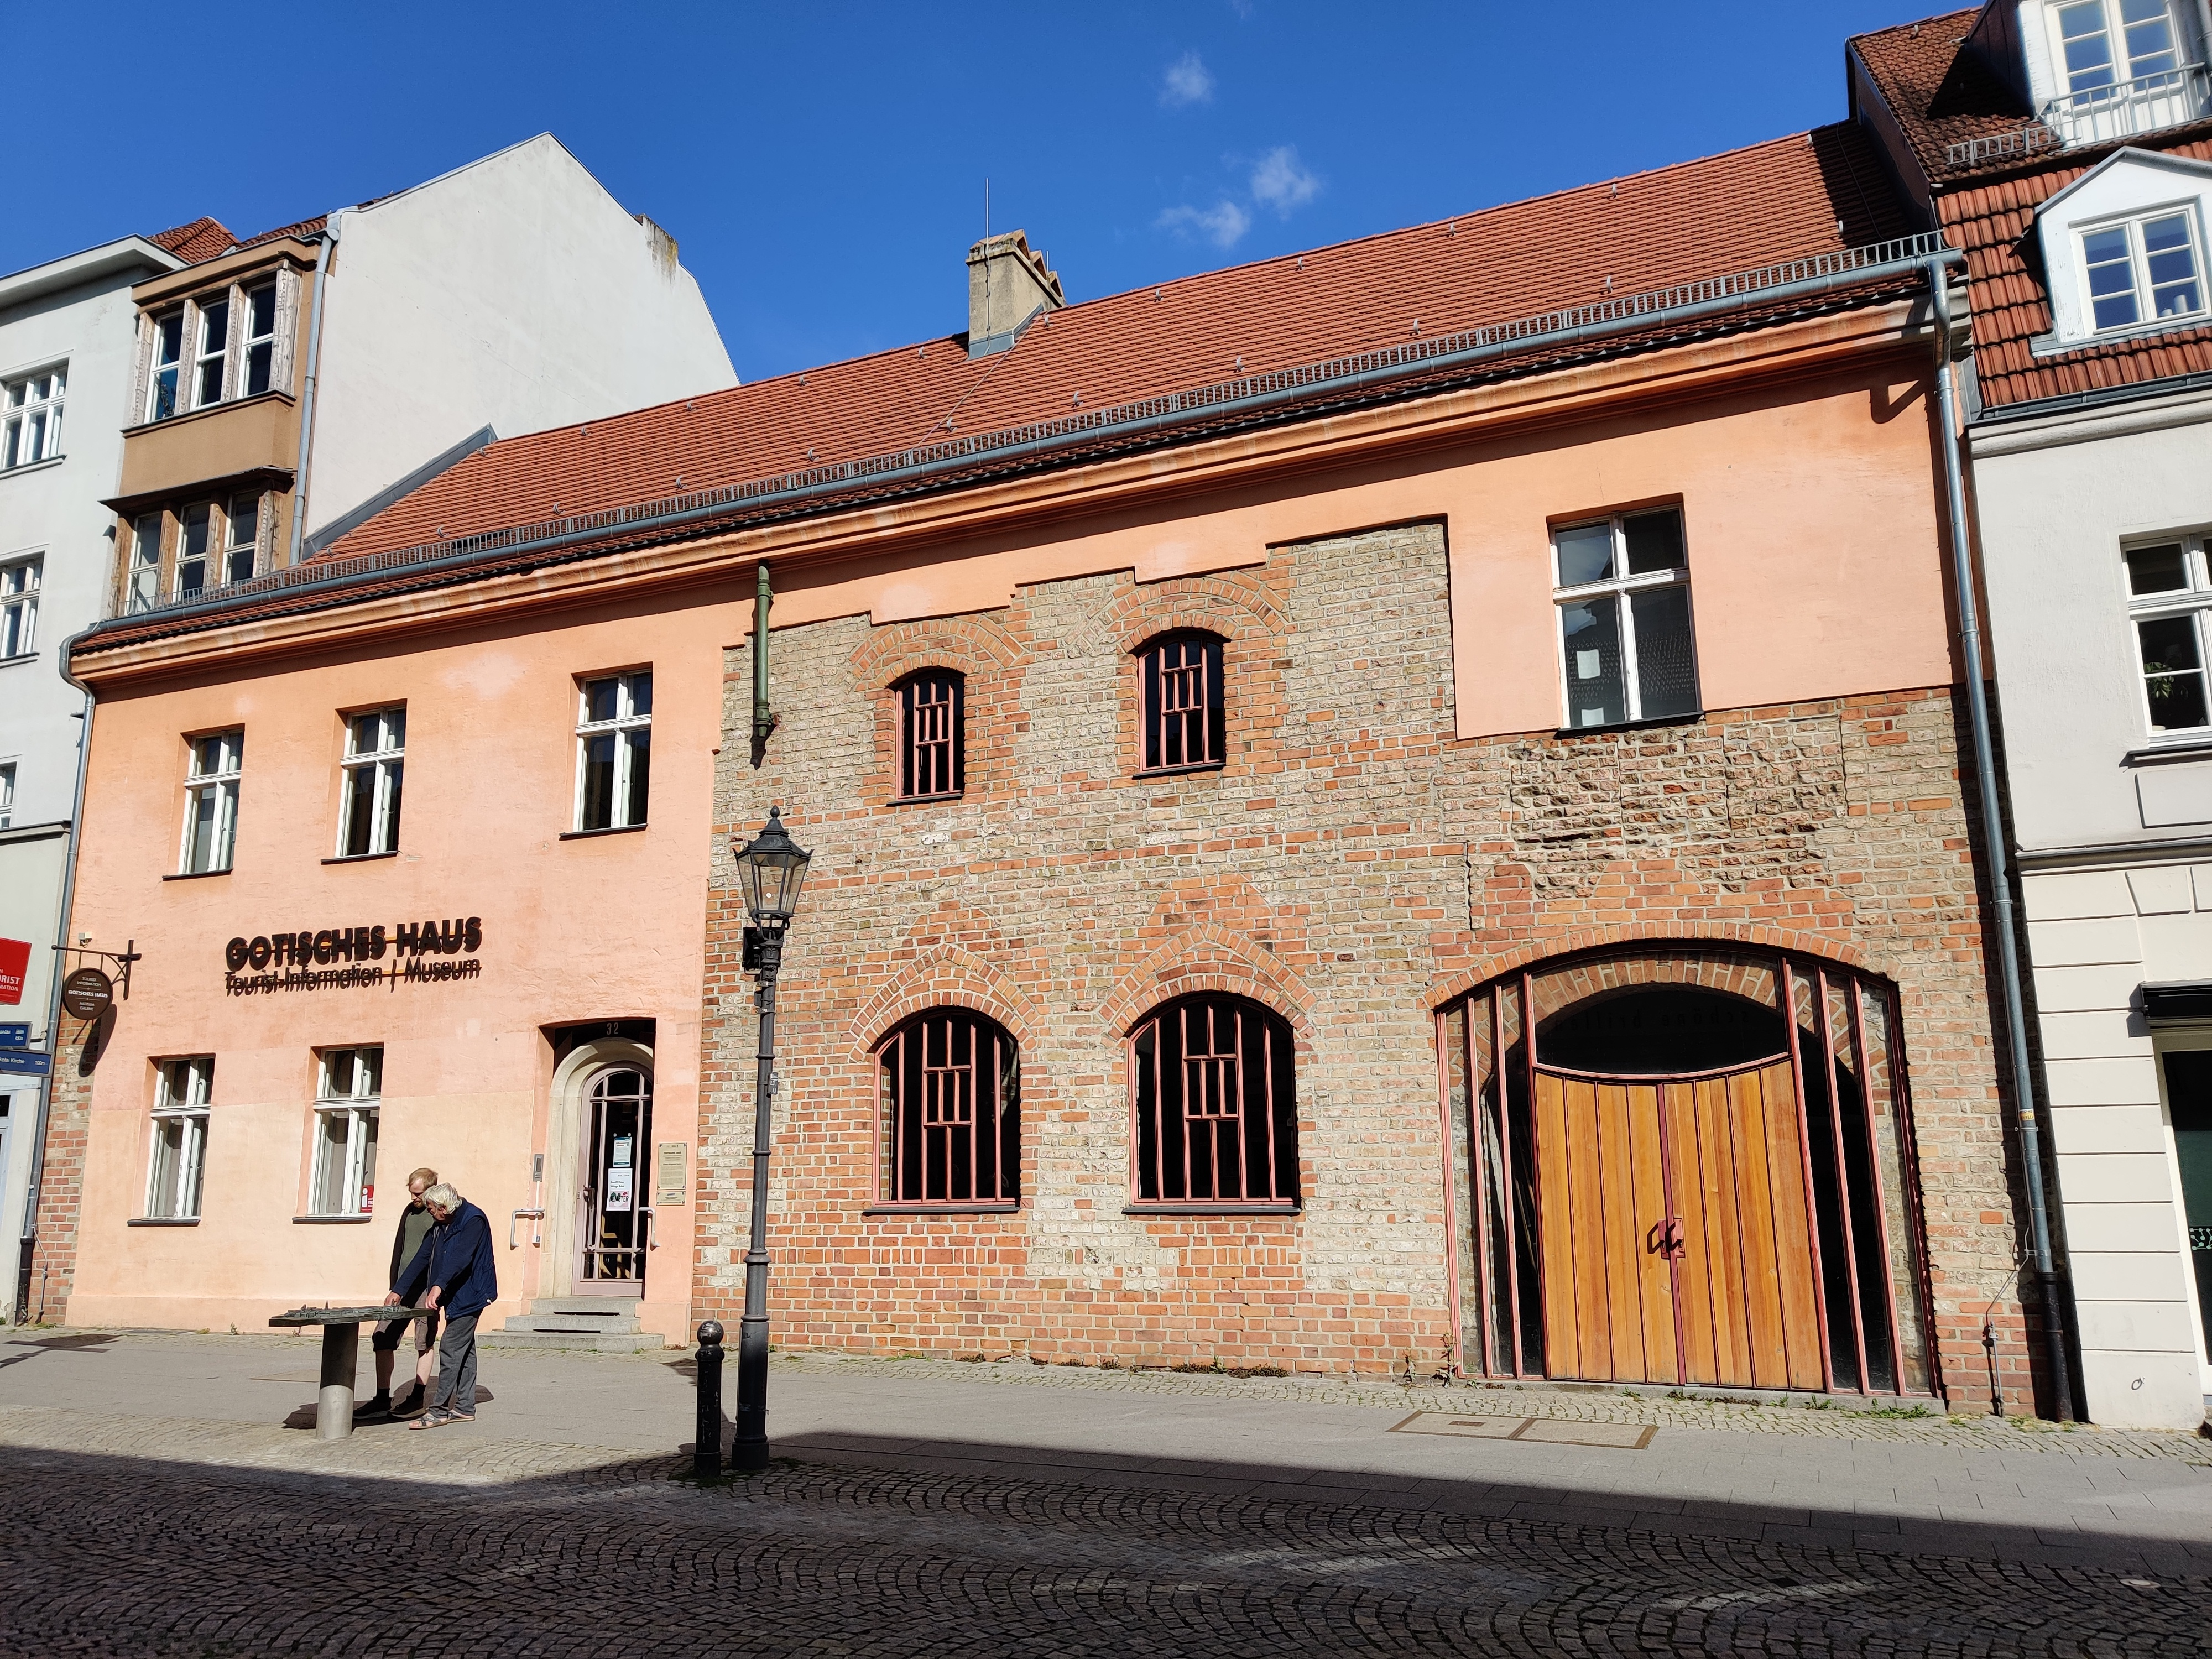
\includegraphics[width=\textwidth]{figures/IMG_20230705_171420.jpg}
        \end{column}
        \begin{column}{0.3\textwidth}
            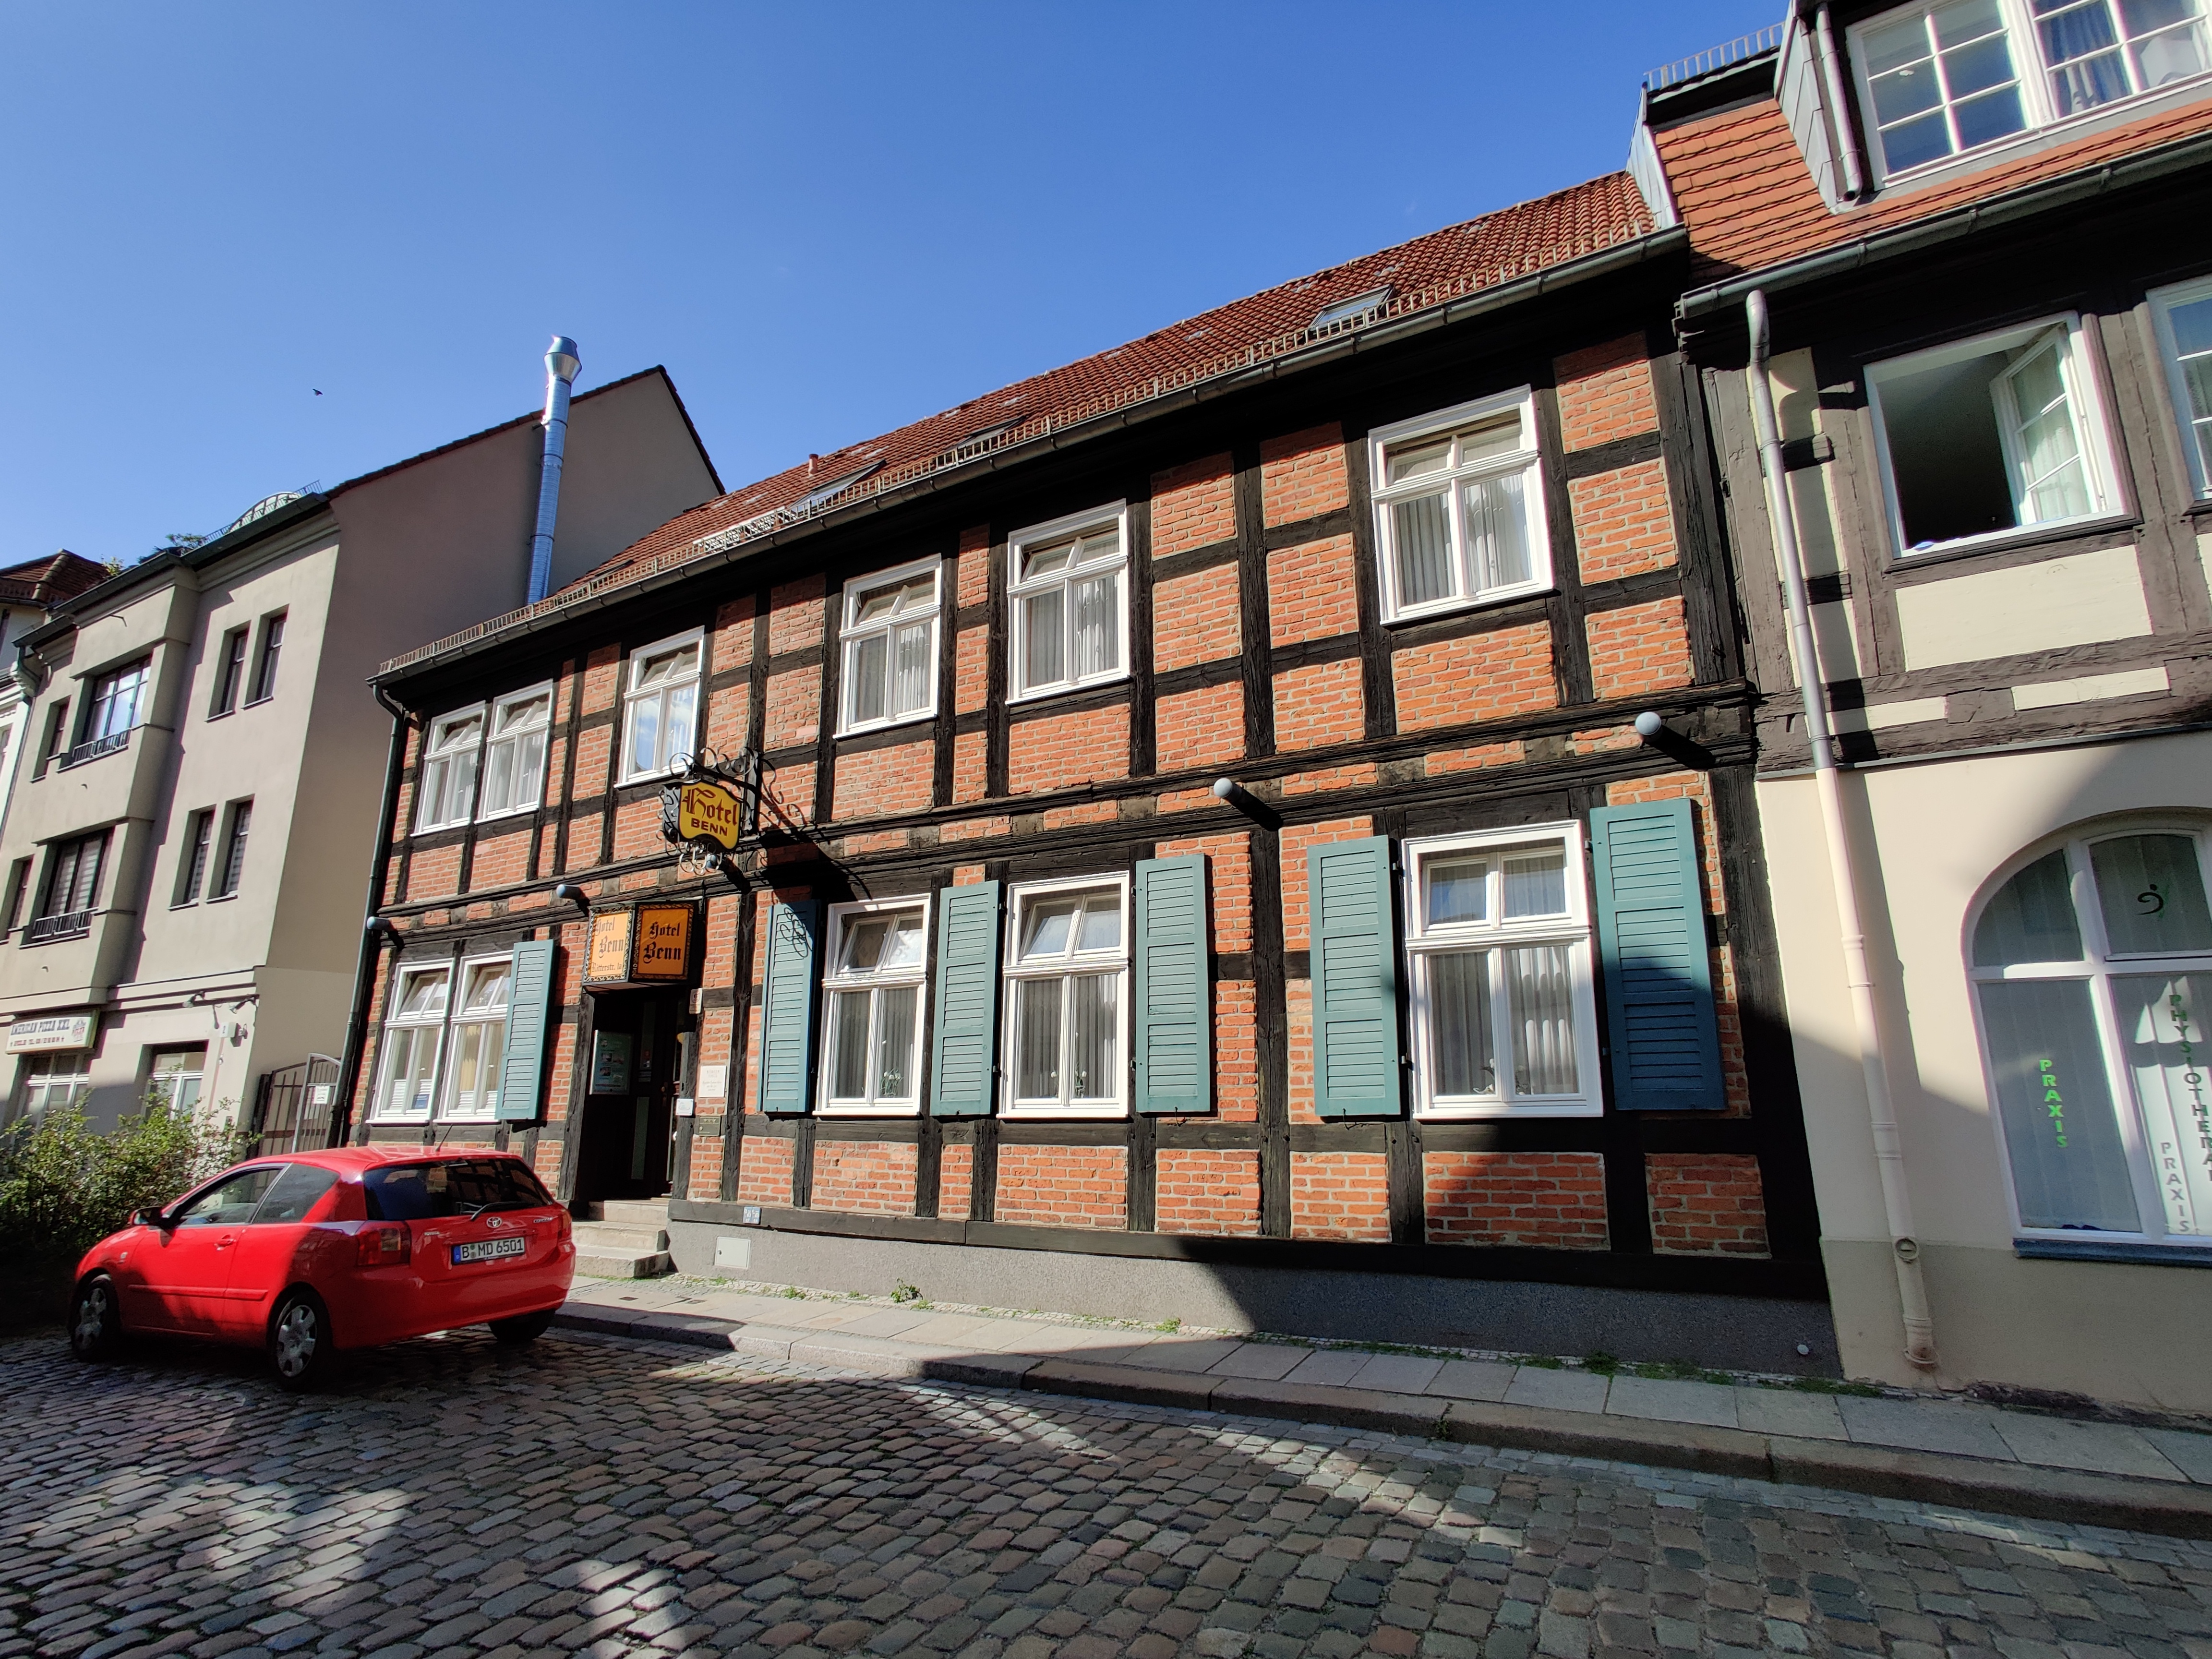
\includegraphics[width=\textwidth]{figures/IMG_20230705_171814.jpg}
        \end{column}
        \begin{column}{0.3\textwidth}
            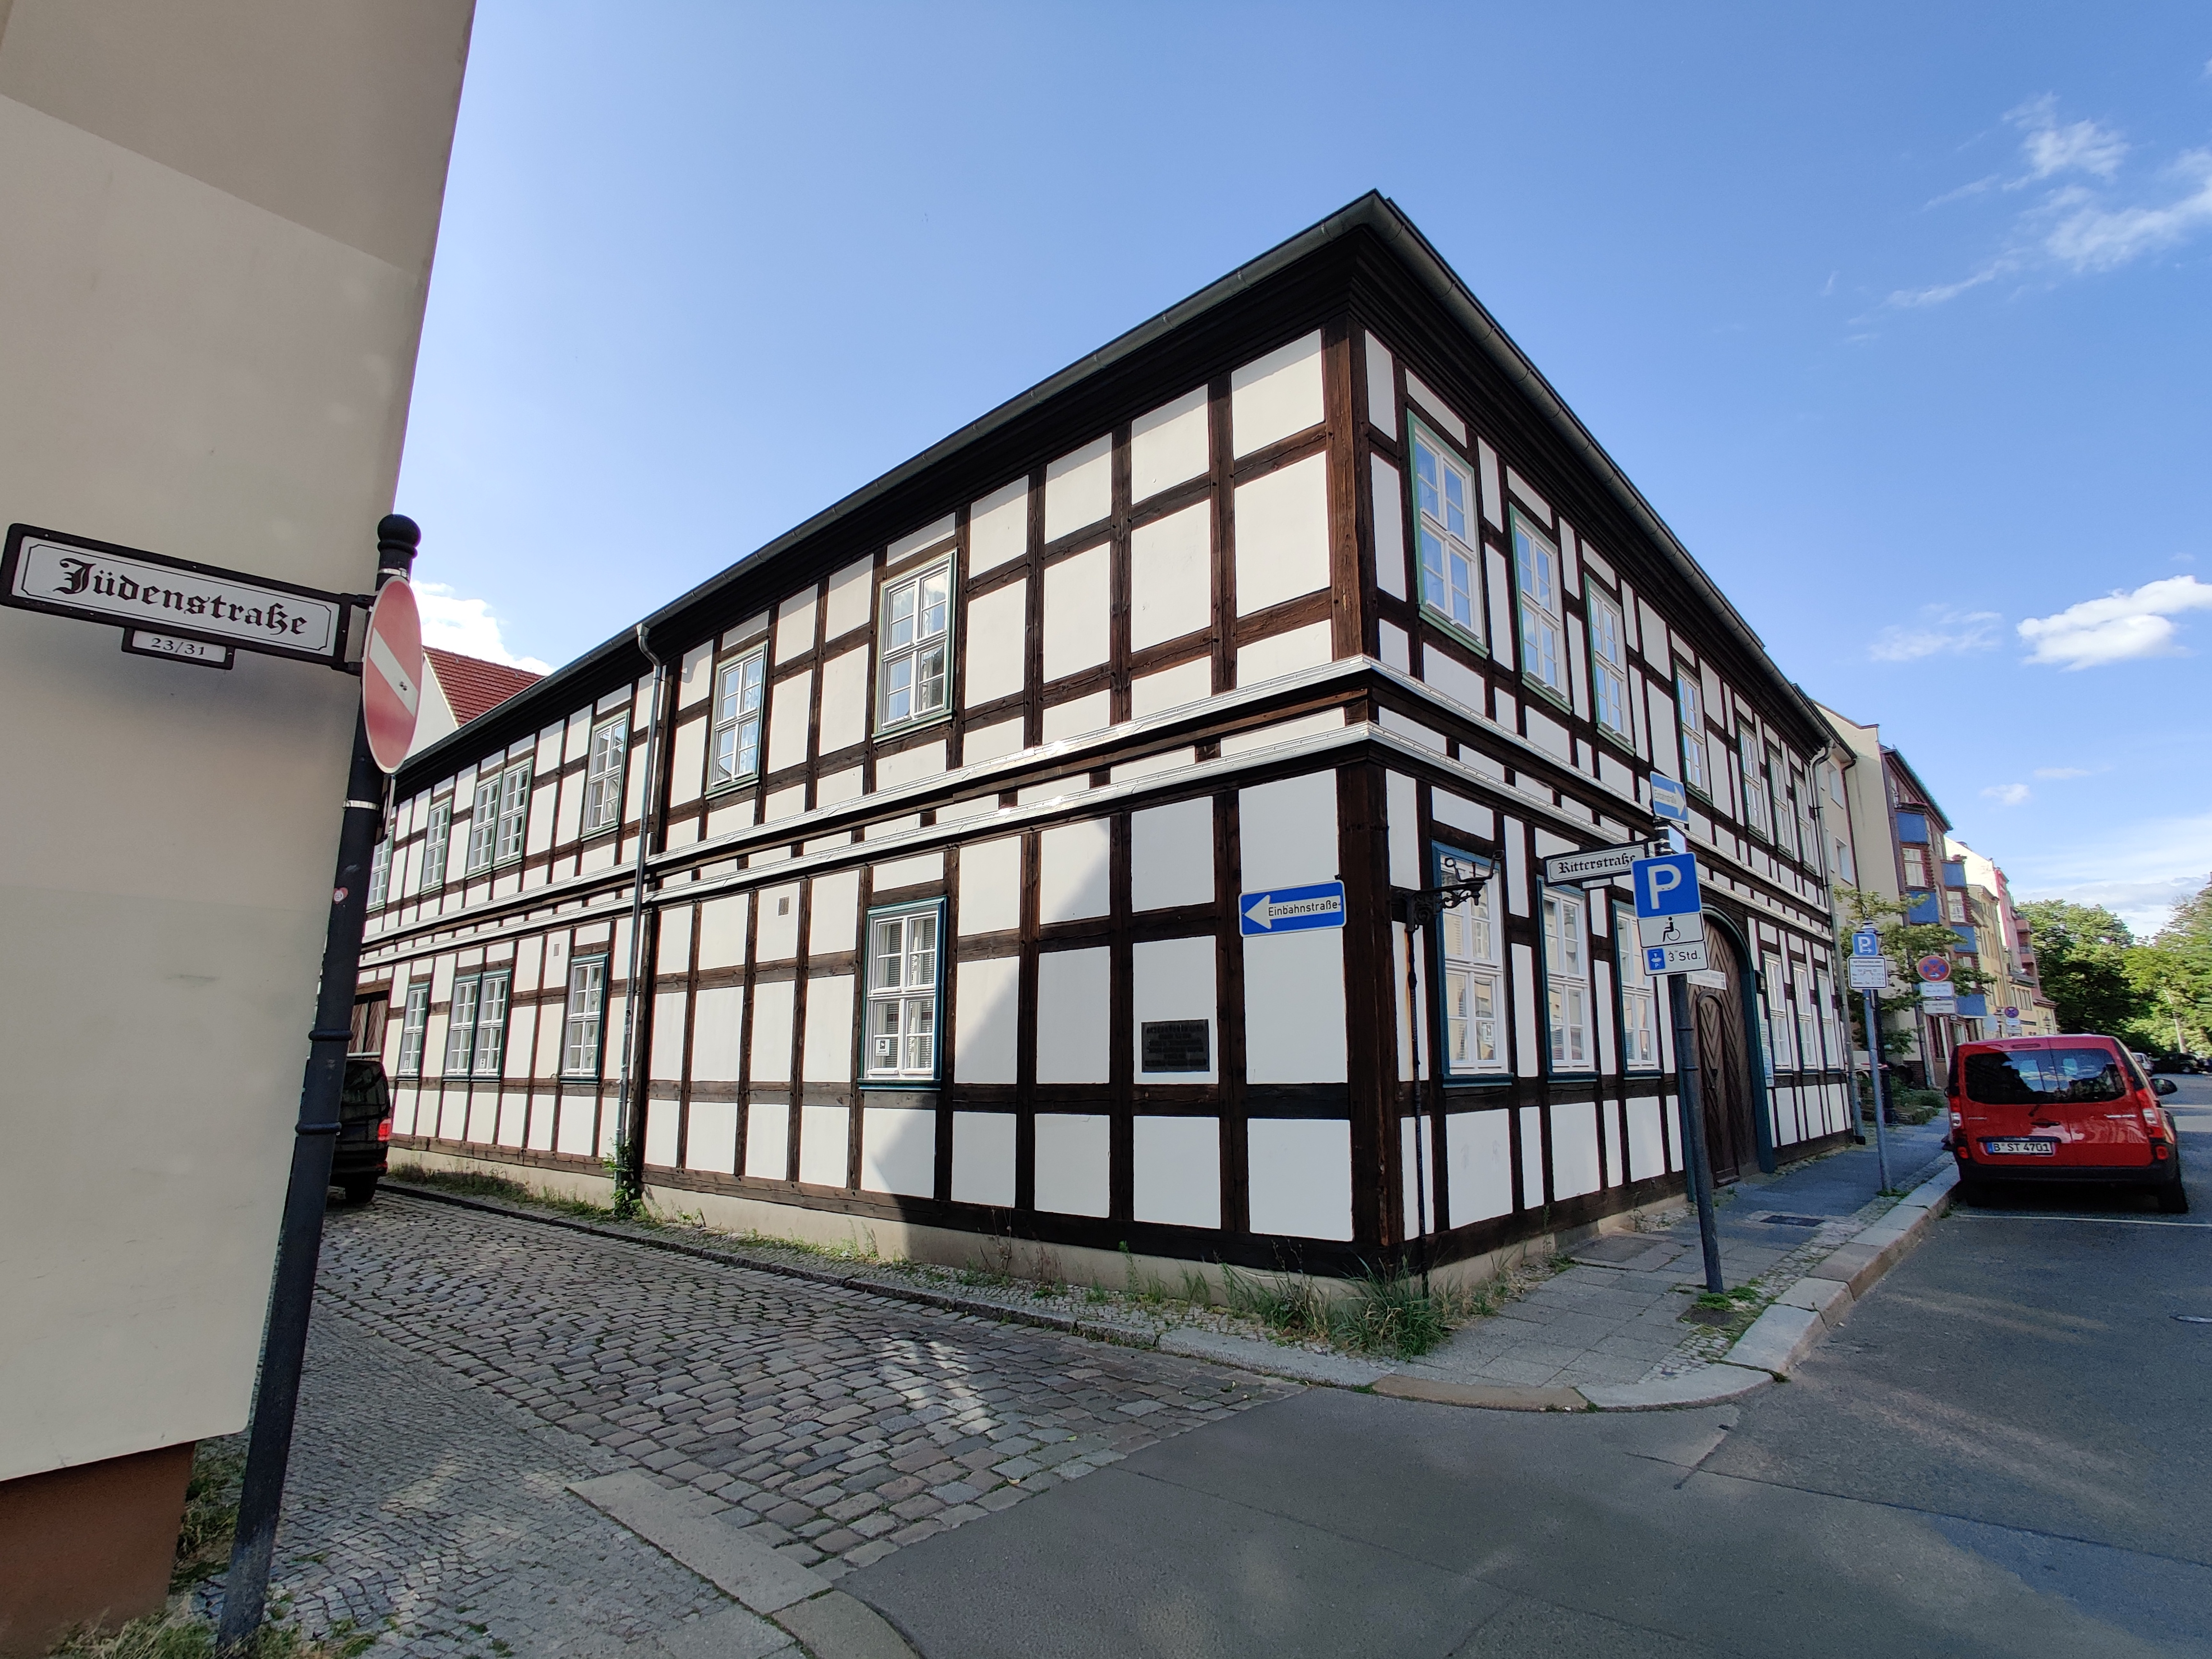
\includegraphics[width=\textwidth]{figures/IMG_20230705_172055.jpg}
        \end{column}
    \end{columns}
    \vspace{0.5cm}
        \begin{columns}
    \begin{column}{0.3\textwidth}
            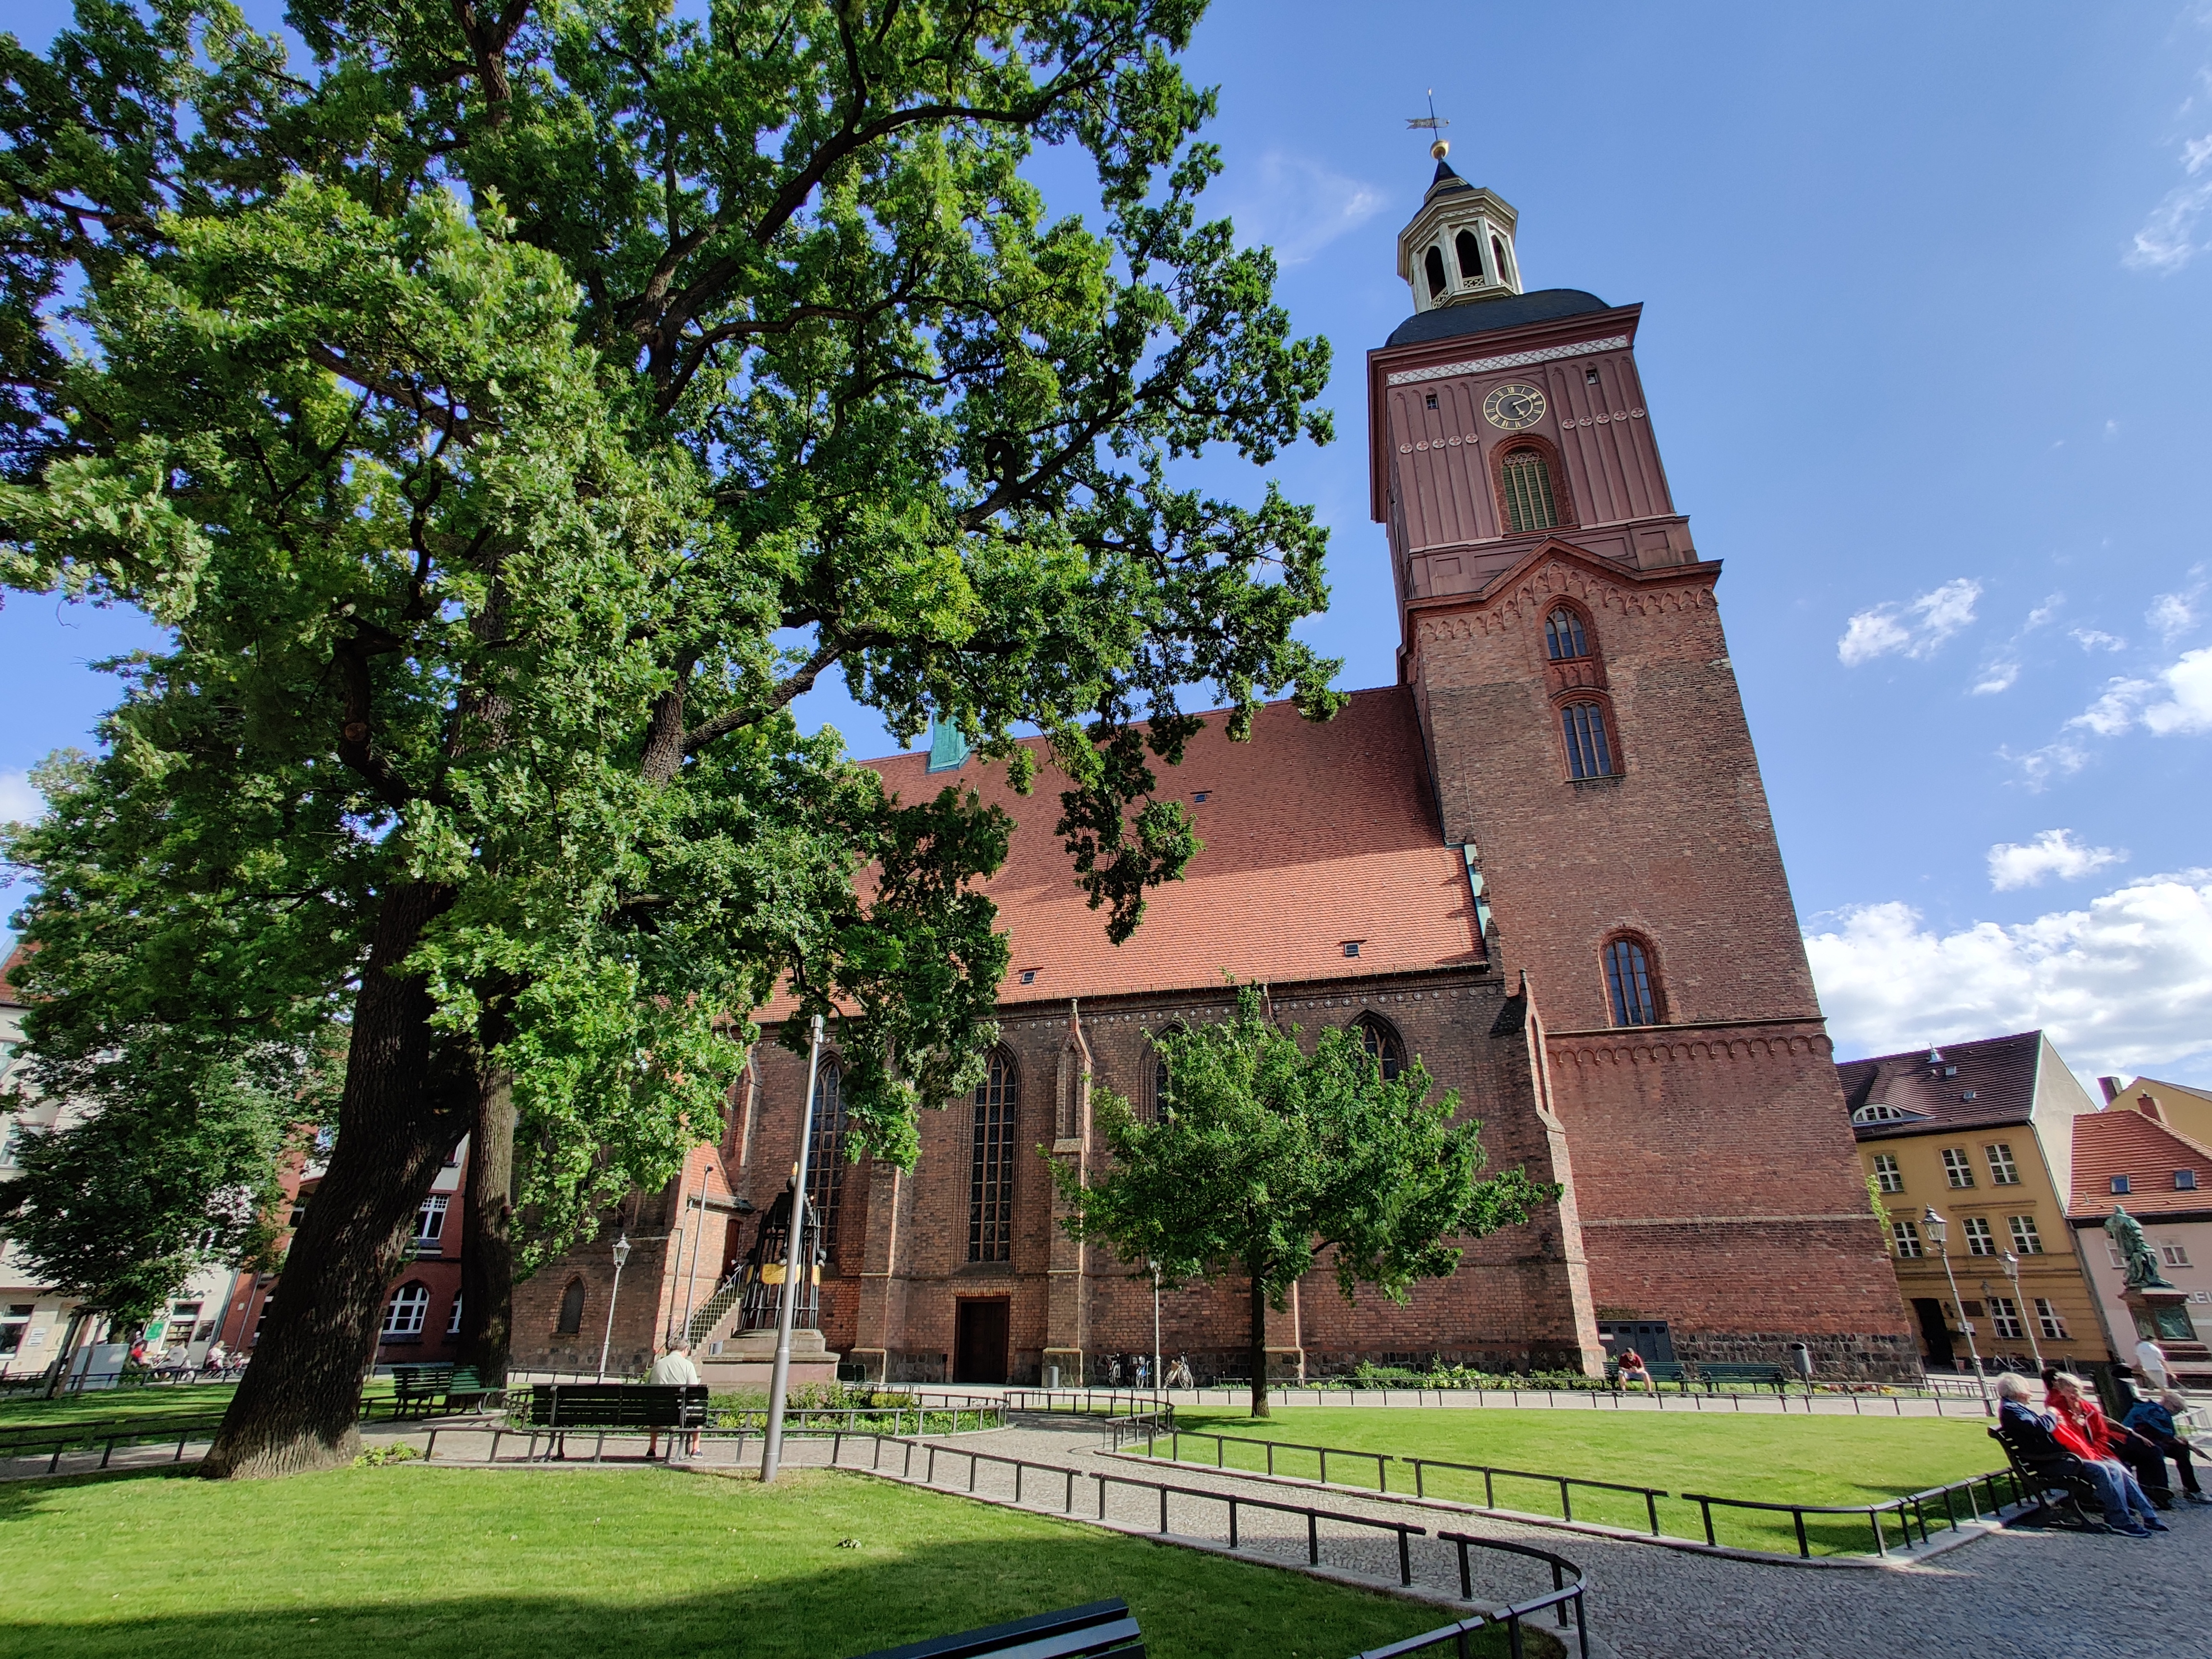
\includegraphics[width=\textwidth]{figures/impressions/IMG_20230705_171154(1).jpg}
        \end{column}
        \begin{column}{0.3\textwidth}
            \includegraphics[width=\textwidth]{figures/impressions/IMG_20230705_173445(1).jpg}
        \end{column}
        \begin{column}{0.3\textwidth}
            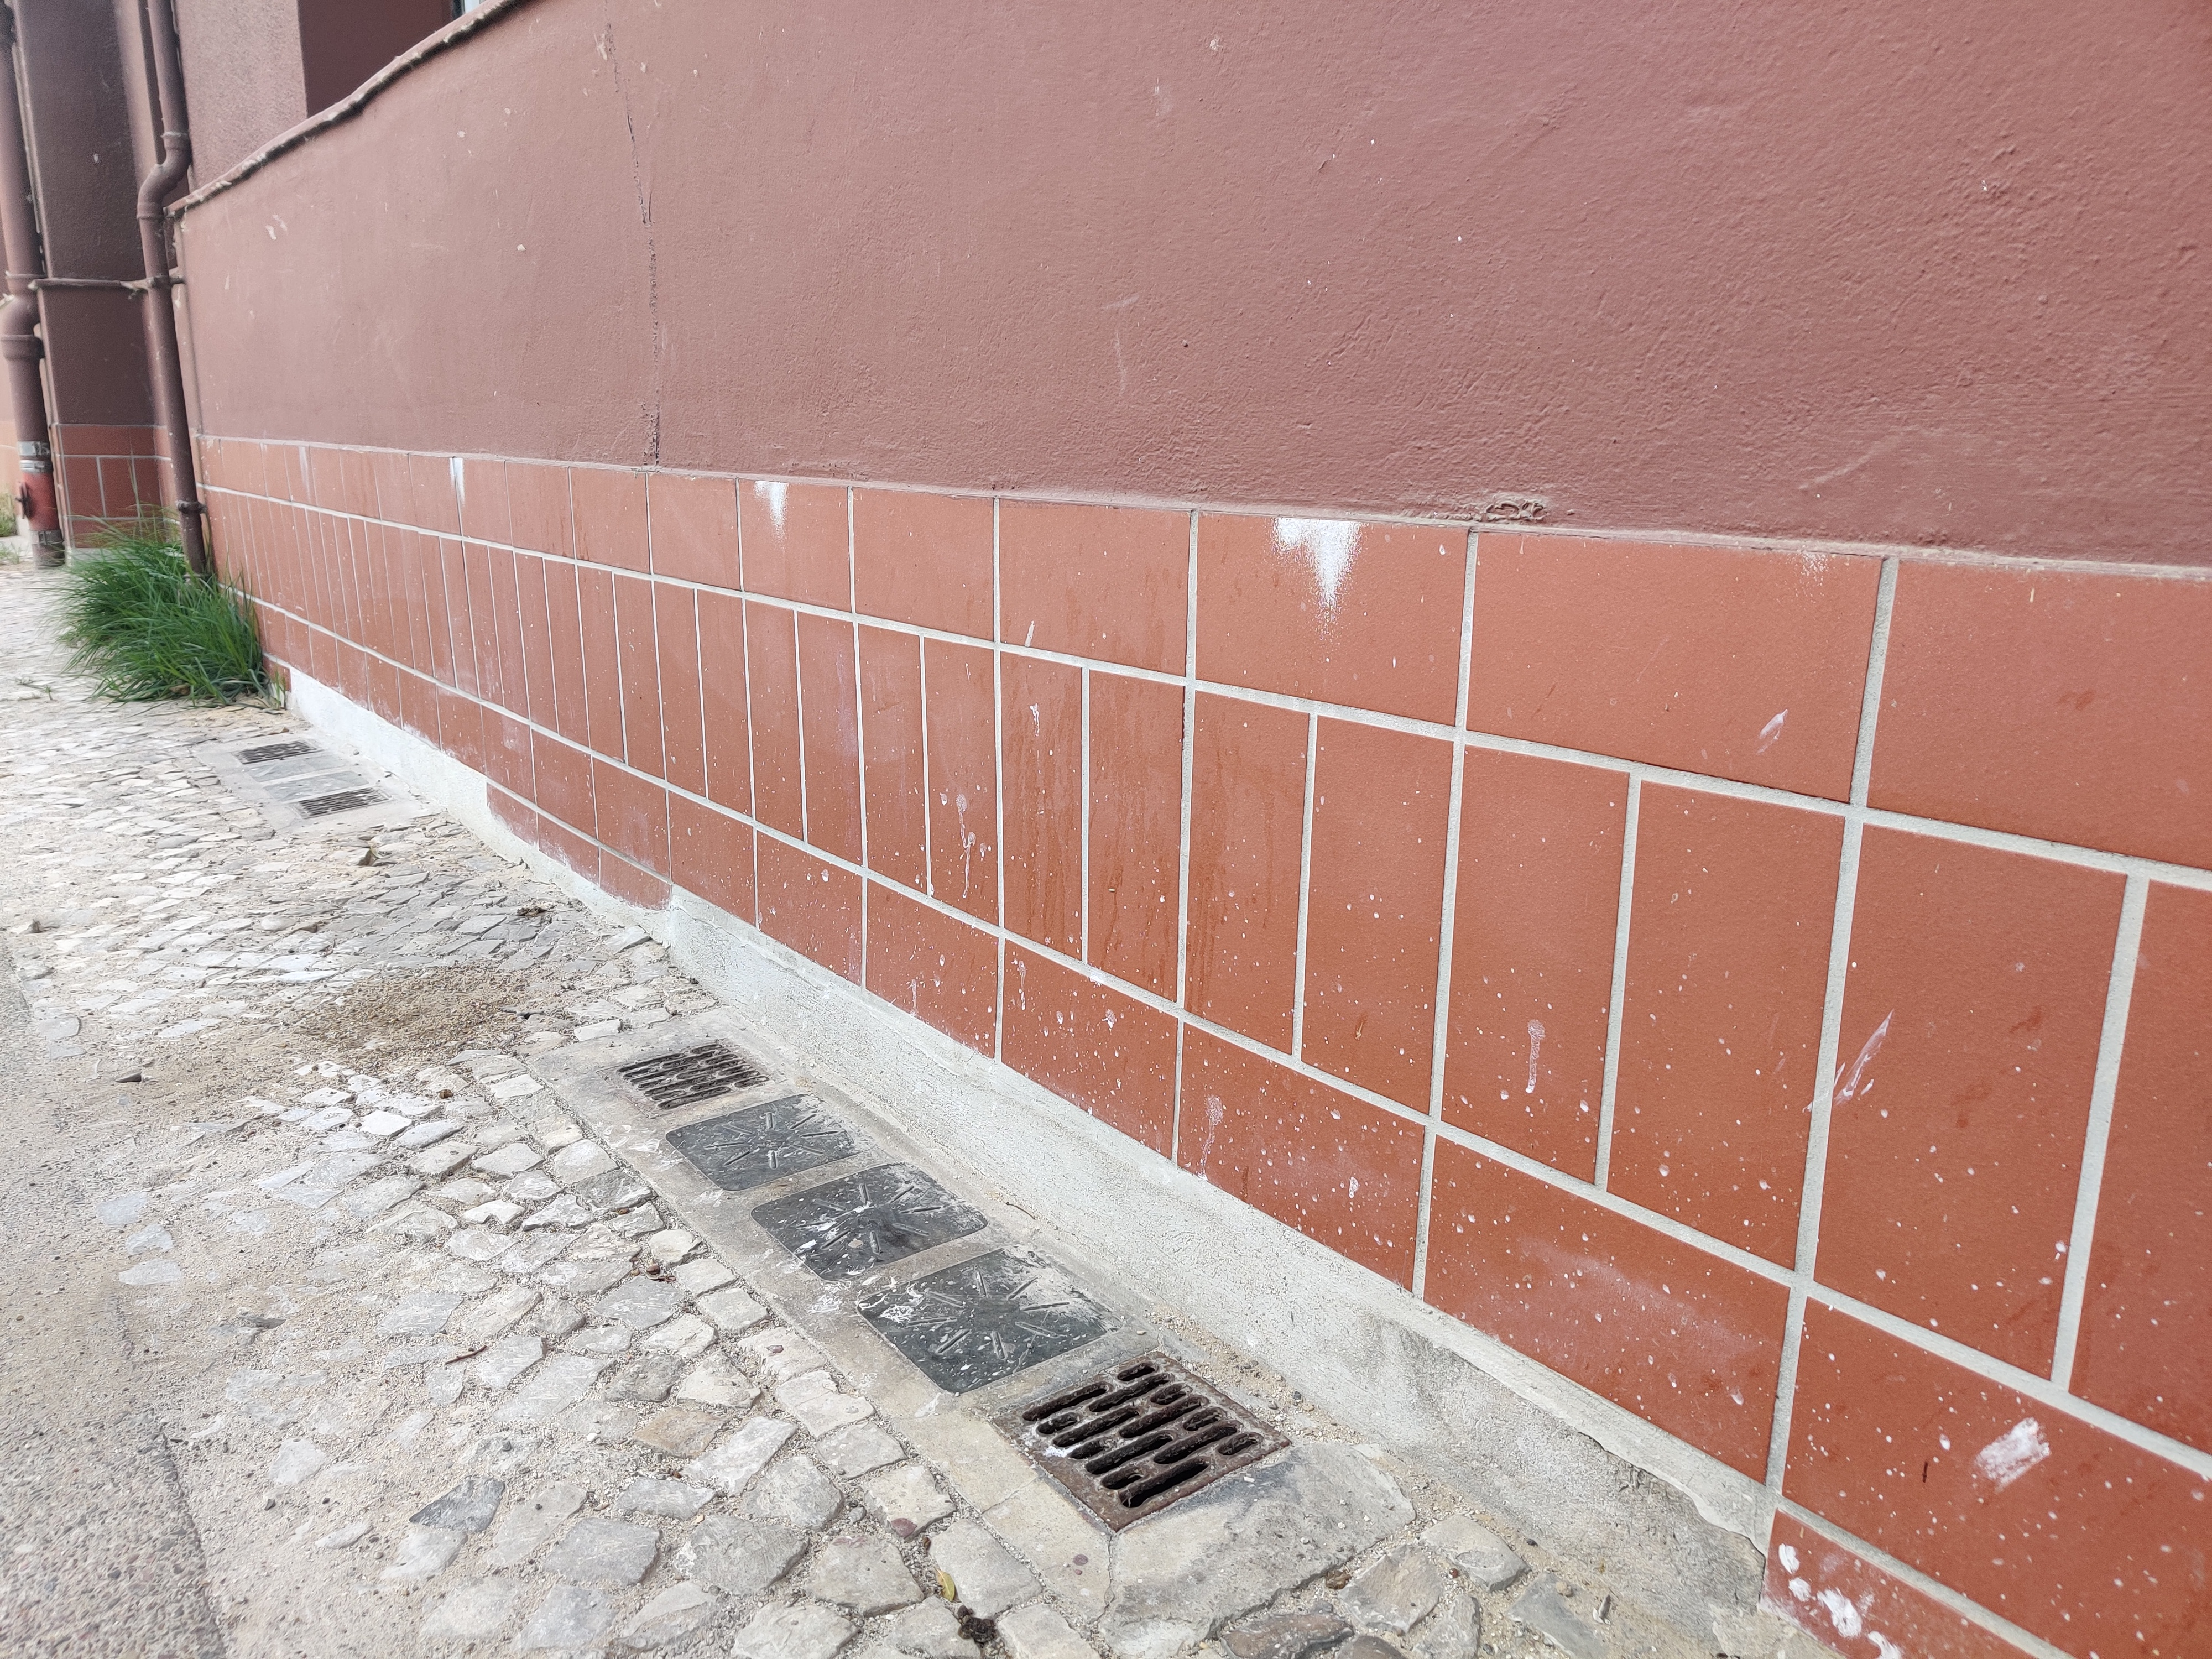
\includegraphics[width=\textwidth]{figures/impressions/IMG_20230705_174427.jpg}
        \end{column}
    \end{columns}
\end{frame}

\section{Zitadelle Spandau}
{ % all template changes are local to this group.
    \setbeamertemplate{navigation symbols}{}
    \begin{frame}<article:0>[plain,noframenumbering]
        \begin{tikzpicture}[remember picture,overlay]
            \node[at=(current page.center)] {
                \includegraphics[
                                 width=\paperwidth,
                                 height=\paperheight]{figures/citadel_section_figure}
            };
        \end{tikzpicture}
    \end{frame}
}

\subsection{History of the Zitadelle Spandau}
\begin{frame}{History}
    \begin{columns}
    % Column 1
    \begin{column}{0.5\textwidth}
            \begin{itemize}
                \item Start of construction 1559 \cite{zitadelleberlin}
                \item Built as a modern fortress
                \item Some buildings taken over from previous castle
                \begin{itemize}
                    \item Partly from the 13th century
                \end{itemize}
            \end{itemize}
    \end{column}
    % Column 2    
    \begin{column}{0.5\textwidth}
        \begin{figure}
        \centering
            \vspace*{-2.5cm}
            \includegraphics[trim= 1200 0 0 0,clip, height=\paperheight]{figures/citadel_outer_view.jpg}
        \end{figure}
    \end{column}
    \end{columns}
\end{frame}

\subsection{Juliusturm}
\begin{frame}{Juliusturm}
    \begin{columns}
    % Column 1
    \begin{column}{0.5\textwidth}
            \begin{itemize}
                \item Built most likely in the 13th century \cite{JostRegina2010DZS-}
                \item changed a lot over the time
                \item mixture of diffenrent bricks and stones
            \end{itemize}
    \end{column}
    % Column 2    
    \begin{column}{0.5\textwidth}
        \begin{figure}
        \centering
            \vspace*{-1.25cm}
            \includegraphics[height=0.9\paperheight]{figures/juliusturm.jpg}
        \end{figure}
    \end{column}
    \end{columns}
\end{frame}

{ % all template changes are local to this group.
    \setbeamertemplate{navigation symbols}{}
    \begin{frame}<article:0>[plain,noframenumbering]
        \begin{tikzpicture}[remember picture,overlay]
            \node[at=(current page.center)] {
                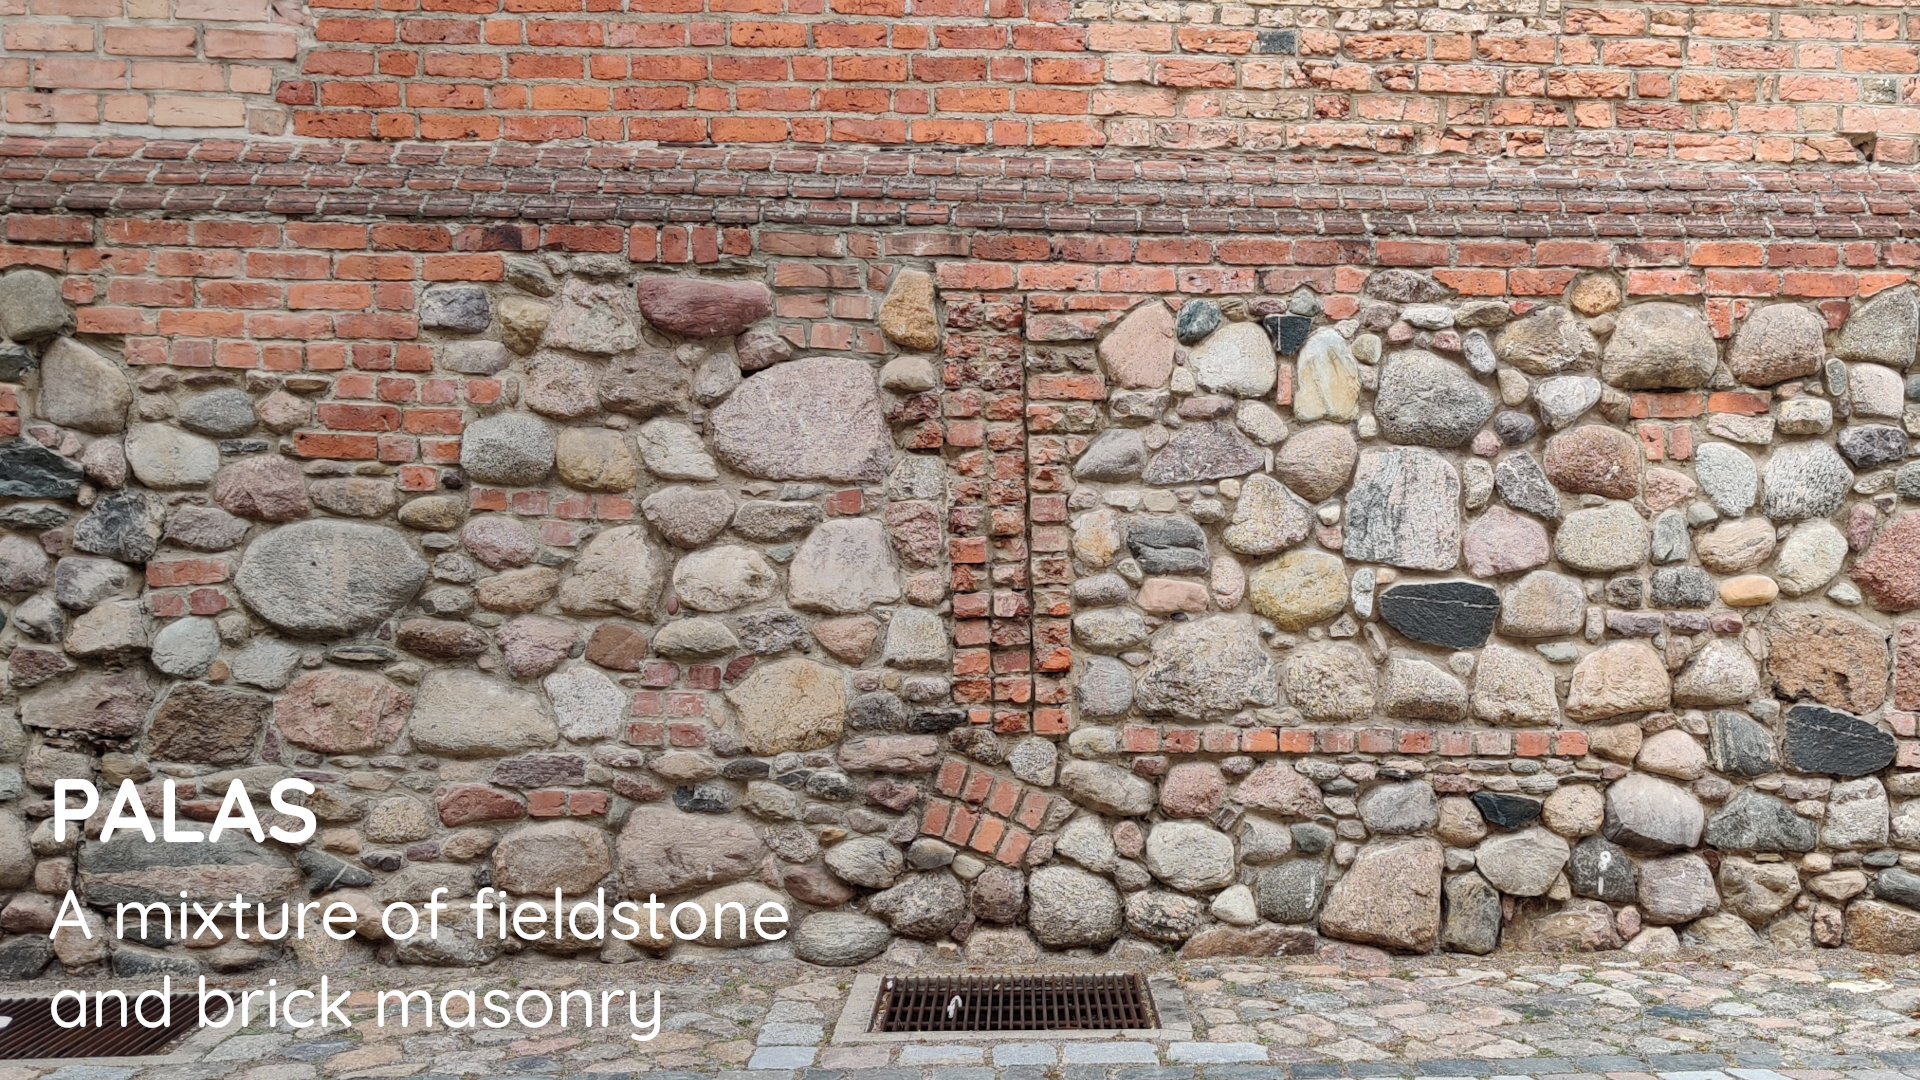
\includegraphics[
                                 width=\paperwidth,
                                 height=\paperheight]{figures/palas_figure}
            };
        \end{tikzpicture}
    \end{frame}
}

{ % all template changes are local to this group.
    \setbeamertemplate{navigation symbols}{}
    \begin{frame}<article:0>[plain,noframenumbering]
        \begin{tikzpicture}[remember picture,overlay]
            \node[at=(current page.center)] {
                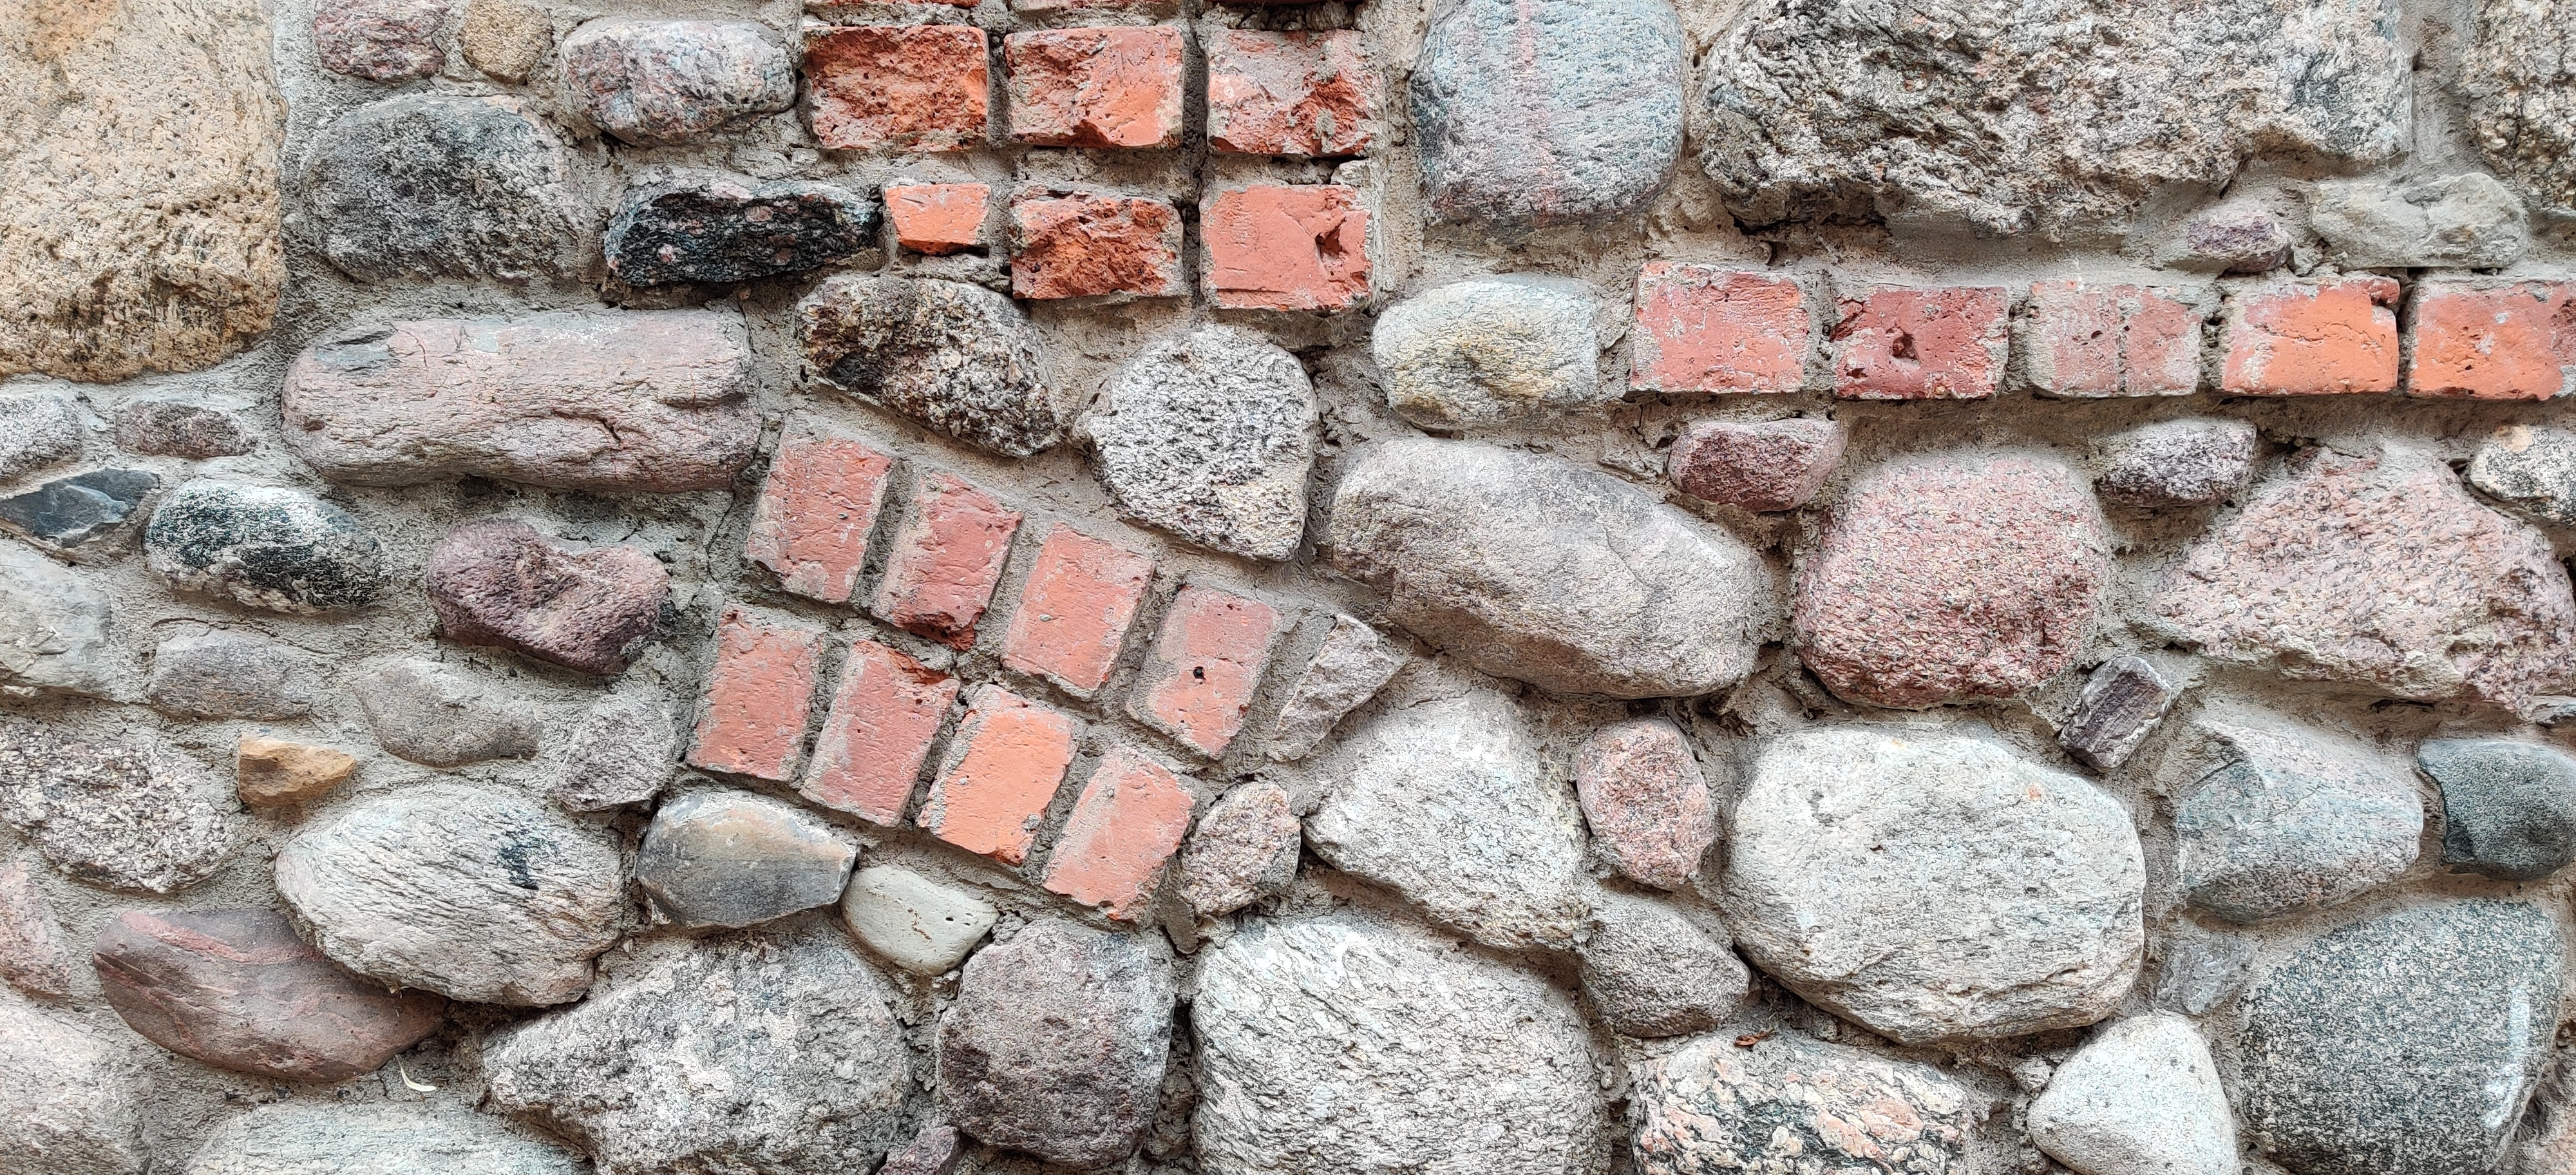
\includegraphics[
                                 width=\paperwidth,
                                 height=\paperheight]{figures/palas_brick_stone_detail}
            };
        \end{tikzpicture}
    \end{frame}
}

\subsection{Zeughaus}
{ % all template changes are local to this group.
    \setbeamertemplate{navigation symbols}{}
    \begin{frame}<article:0>[plain,noframenumbering]
        \begin{tikzpicture}[remember picture,overlay]
            \node[at=(current page.center)] {
                \includegraphics[
                                 width=\paperwidth,
                                 height=\paperheight]{figures/zeughaus}
            };
        \end{tikzpicture}
    \end{frame}
}

\begin{frame}{Zeughaus}
    \begin{columns}
    % Column 1
    \begin{column}{0.5\textwidth}
            \begin{itemize}
                \item Built 1856 - 1858 \cite{visitberlin}
                \item Yellow and red bricks
                \item bricks made in Genthin by Rathenow (Brandenburg, Germany)
            \end{itemize}
    \end{column}
    % Column 2    
    \begin{column}{0.5\textwidth}
        \begin{figure}
        \centering
            \vspace*{-2.5cm}
            \includegraphics[trim= 200 0 0 0,clip,height=\paperheight]{figures/zeughaus.jpg}
        \end{figure}
    \end{column}
    \end{columns}
\end{frame}

\subsection{Zeughaus}
{ % all template changes are local to this group.
    \setbeamertemplate{navigation symbols}{}
    \begin{frame}<article:0>[plain,noframenumbering]
        \begin{tikzpicture}[remember picture,overlay]
            \node[at=(current page.center)] {
                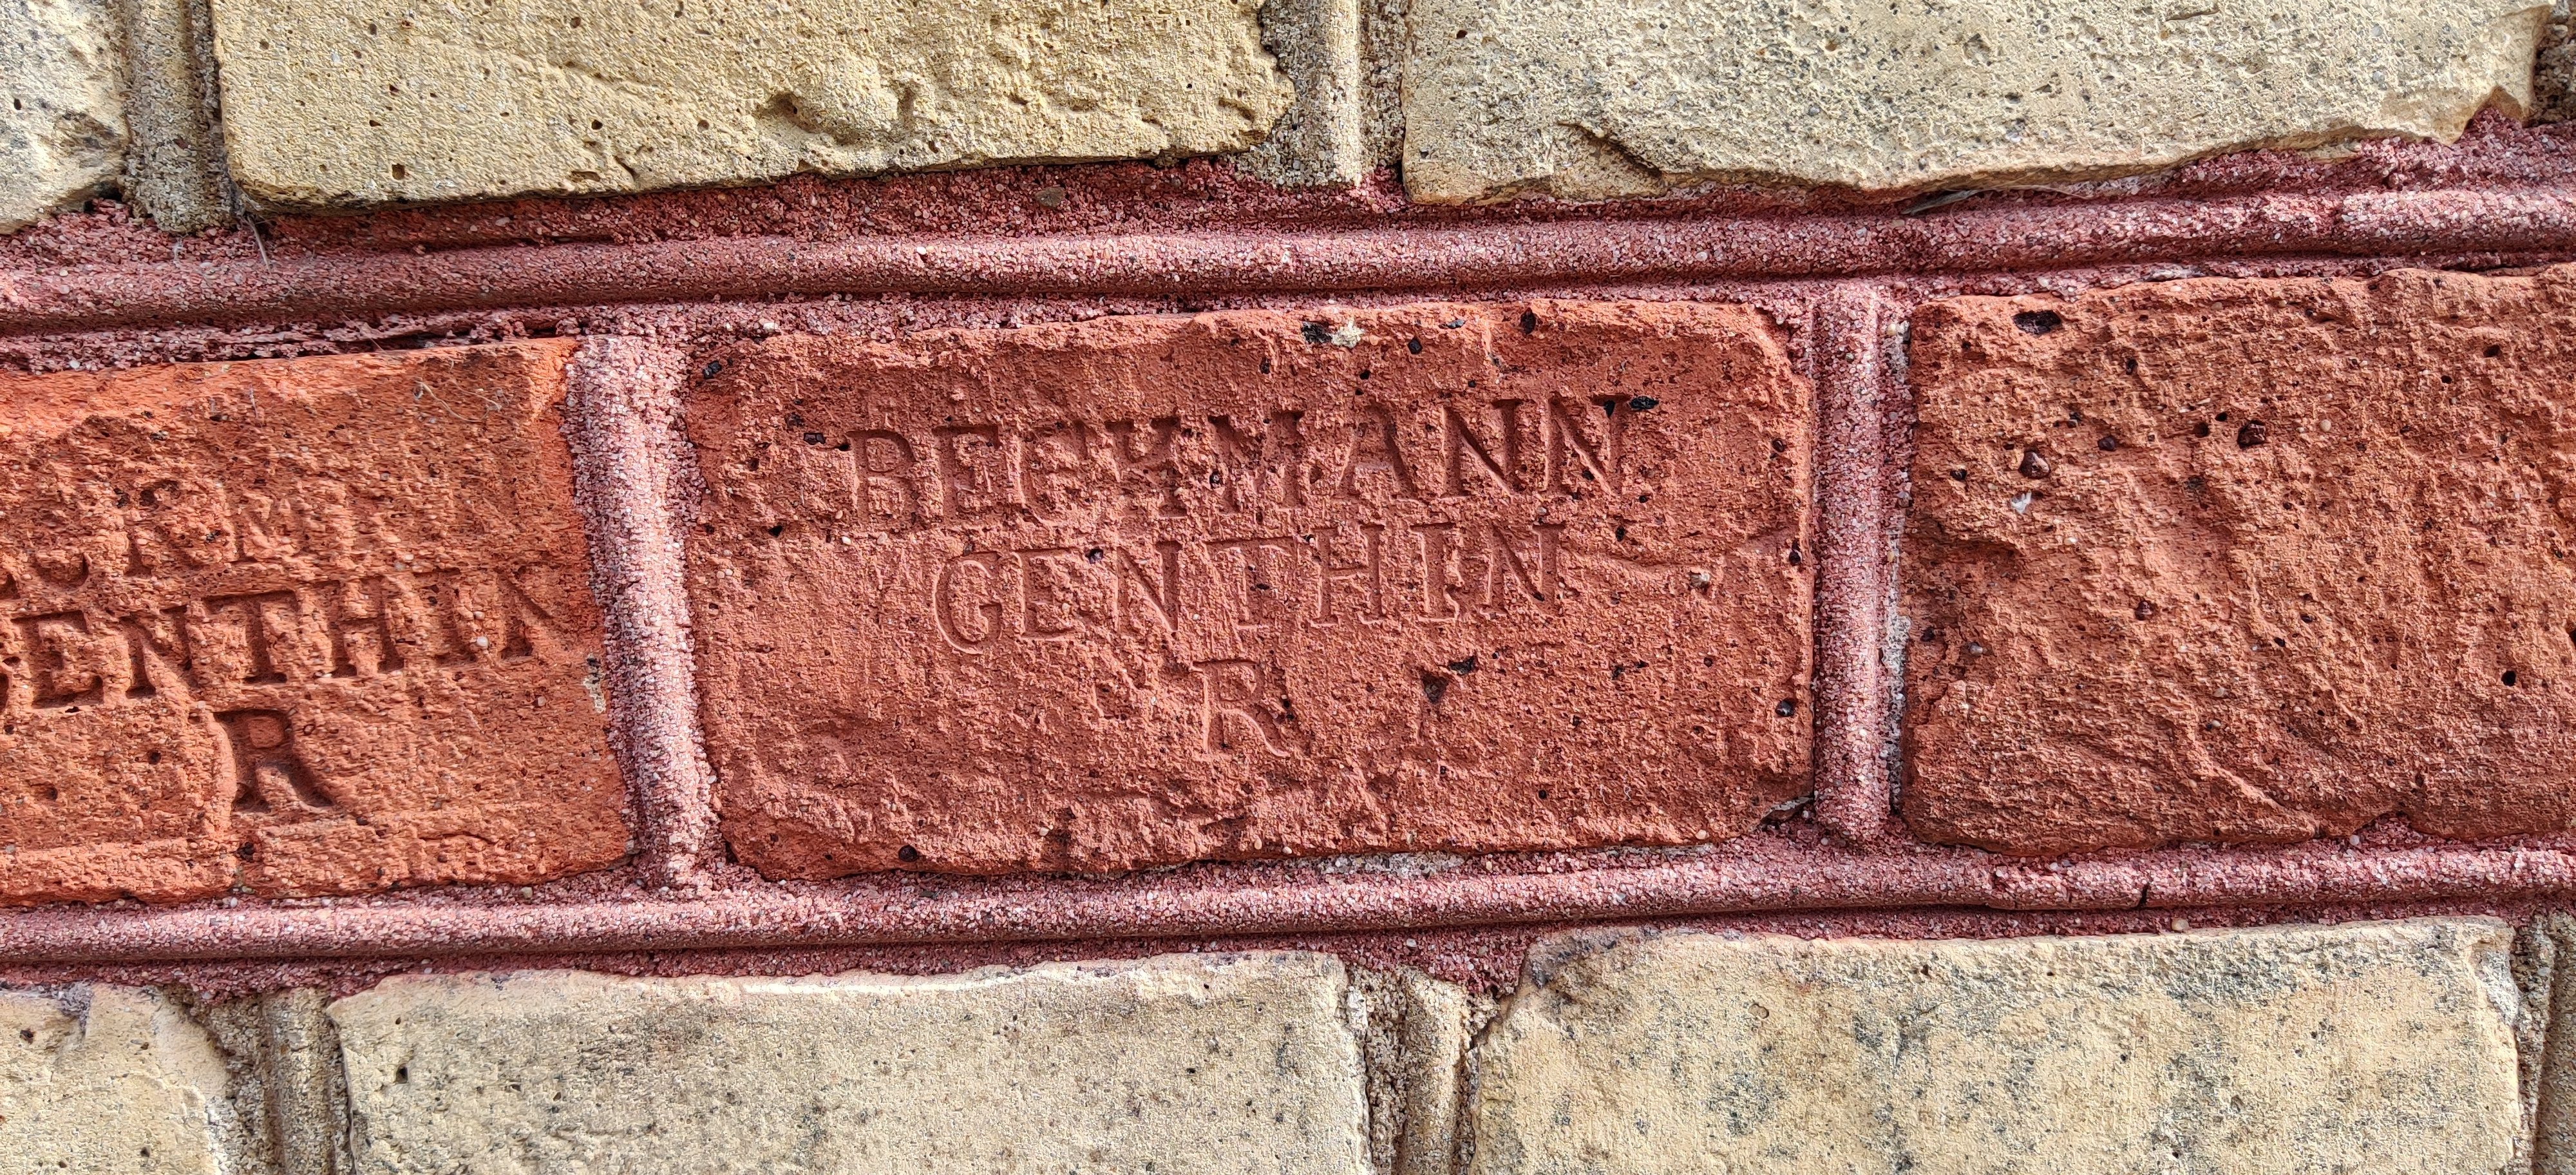
\includegraphics[
                                 width=\paperwidth,
                                 height=\paperheight]{figures/zeughaus_detail}
            };
        \end{tikzpicture}
    \end{frame}
}

\begin{frame}
    \frametitle{Zeughaus | Bricks origin}
    \framesubtitle{}
    \vspace{5mm}
    \begin{figure}
        \centering
            \includegraphics[height=0.65\paperheight]{figures/maps/map_genthin.png}
            \caption{Map of Genthin and Rathenow. Distance between Genthin and Zitadelle about 75 km. \cite{OpenStreetMap}}
        \label{fig:enter-label}
    \end{figure}
\end{frame}

\section{Degradation}

\subsection{Degradation}
{ % all template changes are local to this group.
    \setbeamertemplate{navigation symbols}{}
    \begin{frame}<article:0>[plain,noframenumbering]
        \begin{tikzpicture}[remember picture,overlay]
            \node[at=(current page.center)] {
                \includegraphics[
                                 width=\paperwidth,
                                 height=\paperheight]{figures/degradation_section_figure}
            };
        \end{tikzpicture}
    \end{frame}
}

\begin{frame}
    \frametitle{Degradation}
    \vspace{5mm}
    \begin{figure}
        \centering
            \includegraphics[height=0.65\paperheight]{figures/bastion_degradation.jpg}
            \caption{The outer walls were faced in the 19th century to hide the damage of the past. \cite{JostRegina2010DZS-}}
        \label{fig:enter-label}
    \end{figure}
\end{frame}

\begin{frame}
    \frametitle{Degradation}
    \vspace{5mm}
    \begin{figure}
        \centering
            \includegraphics[height=0.65\paperheight]{figures/degradation_bricks.jpg}
            \caption{Stains on bricks at the building next to the Juliusturm}
        \label{fig:enter-label}
    \end{figure}
\end{frame}

{ % all template changes are local to this group.
    \setbeamertemplate{navigation symbols}{}
    \begin{frame}<article:0>[plain,noframenumbering]
        \begin{tikzpicture}[remember picture,overlay]
            \node[at=(current page.center)] {
                \includegraphics[
                                 width=\paperwidth,
                                 height=\paperheight]{figures/archway}
            };
        \end{tikzpicture}
    \end{frame}
}

\begin{frame}
    \frametitle{Degradation}
    \vspace{5mm}
    \begin{figure}
        \centering
            \includegraphics[height=0.65\paperheight]{figures/white_inside_zeughaus.jpg}
            \caption{The yellow stones from the armoury have a white discolouration inside.}
        \label{fig:enter-label}
    \end{figure}
\end{frame}

\section*{Bibliography}
\begin{frame}[fragile]{Bibliography}

\printbibliography
\end{frame}

\appendix

\begin{frame}{Thank you!}
    \framesubtitle{Download presentation and all images}
    \vspace{0.5in}
    \centering
    \qrcode[height=2in]{https://github.com/2481632/Ceramics-for-my-built-environment}
\end{frame}

\end{document}
